\documentclass[14pt]{extarticle}
\usepackage[english, russian]{babel}
\usepackage[left=20mm, right=10mm, top=20mm, bottom=20mm]{geometry}
\usepackage{graphicx}
\usepackage{titlesec}
\usepackage{array}
\usepackage{wrapfig}
\usepackage{color, colortbl}
\usepackage[colorlinks=true,linkcolor=cyan,unicode=true]{hyperref}
\usepackage{mathtools}
\usepackage{setspace}
\usepackage{svg}
 
\newcommand\ddformula[1]{\displaystyle #1}
 
\titleformat{\section}
  {\normalfont\fontsize{14}{16}\bfseries}{\thesection}{0.5em}{}
 
\begin{document}
    \begin{minipage}{0.5\textwidth}
        \begin{center}
            \begin{small}
                \textsf{\textbf{Университет ИТМО}} \\
                \textsf{\textbf{Физико-технический мегафакультет}} \\
                \textsf{\textbf{Физический факультет}}
            \end{small}
        \end{center}
    \end{minipage}
    \hfill
    \begin{minipage}{0.4\textwidth}
        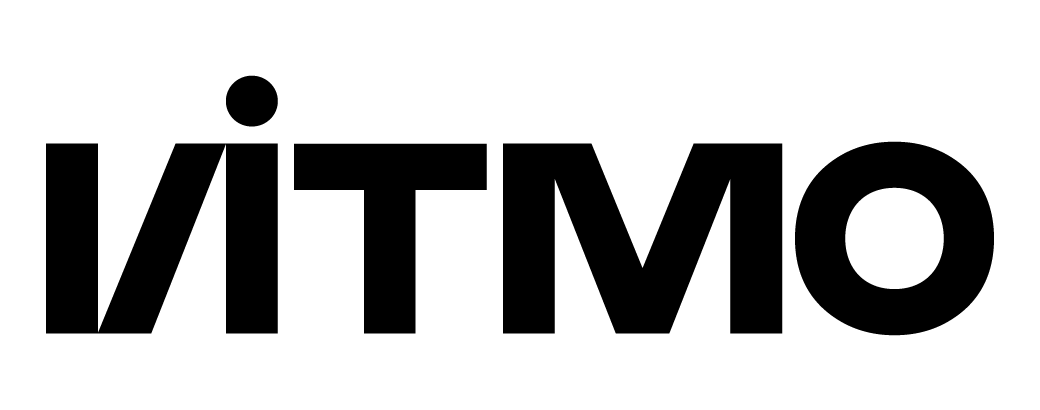
\includegraphics[height=2.5cm]{itmo.png}
    \end{minipage}
    \hrule
    \vspace{8mm}
    \begin{minipage}{0.4\textwidth}
        Группа:  \\ % ГРУППА
        Студент:  \\ % СТУДЕНТ
        Преподаватель: Смирнов А.В % ПРЕПОД
    \end{minipage}
    \hfill
    \begin{minipage}{0.4\textwidth}
        К работе допущен: \\
        Работа выполнена: \\
        Отчёт принят: 
    \end{minipage}
    \vspace{8mm}
    \begin{center}
        \begin{Large}
            \textbf{Рабочий протокол и отчёт по лабораторной работе №} \\ % УКАЗАТЬ НОМЕР ЛАБЫ
            Определение удельного заряда электрона % УКАЗАТЬ НАЗВАНИЕ ЛАБЫ
        \end{Large}
    \end{center}
    \vspace{8mm}
 
    \section{Цель работы}
    
    \section{Задачи, решаемые при выполнении работы}
    
    \section{Объект исследования}
    
    \section{Метод экспериментального исследования}
    
    \section{Рабочие формулы и исходные данные}

    \section{Измерительные приборы}

    \section{Схема установки}

    \section{Расчёт результатов косвенных изменений}

    \section{Расчёт погрешностей изменений}
 
    \section{Графики}

    \section{Окончательные результаты}

    \section{Вывод и анализ результатов}

    \end{document}